\documentclass{beamer}
\usepackage{./external_pkgs/physics/physics}
\usepackage [theme=default]{./external_pkgs/jlcode /jlcode}
\usepackage{graphicx}
\title{Title}
\author{MK}
\institute{}
\date{Date}

\begin{document}
	\frame{\titlepage}
	\begin{frame}
		\frametitle{Table of Contents}
		\tableofcontents
	\end{frame}
\section{Basic Slide with Items}
\begin{frame}{Slide Title}
	\framesubtitle{slide subtitle}
	\begin{itemize}
		\item item
	\end{itemize}
\end{frame}	
\section{Columns}
\begin{frame}
	\frametitle{Using Columns}
	\begin{columns}
		\column{0.5\textwidth}
		<text>
		\column{0.5\textwidth}
		<text>
	\end{columns}
\end{frame}


\section{Figures}
\begin{frame}	
\frametitle{Figures}
\begin{figure}
	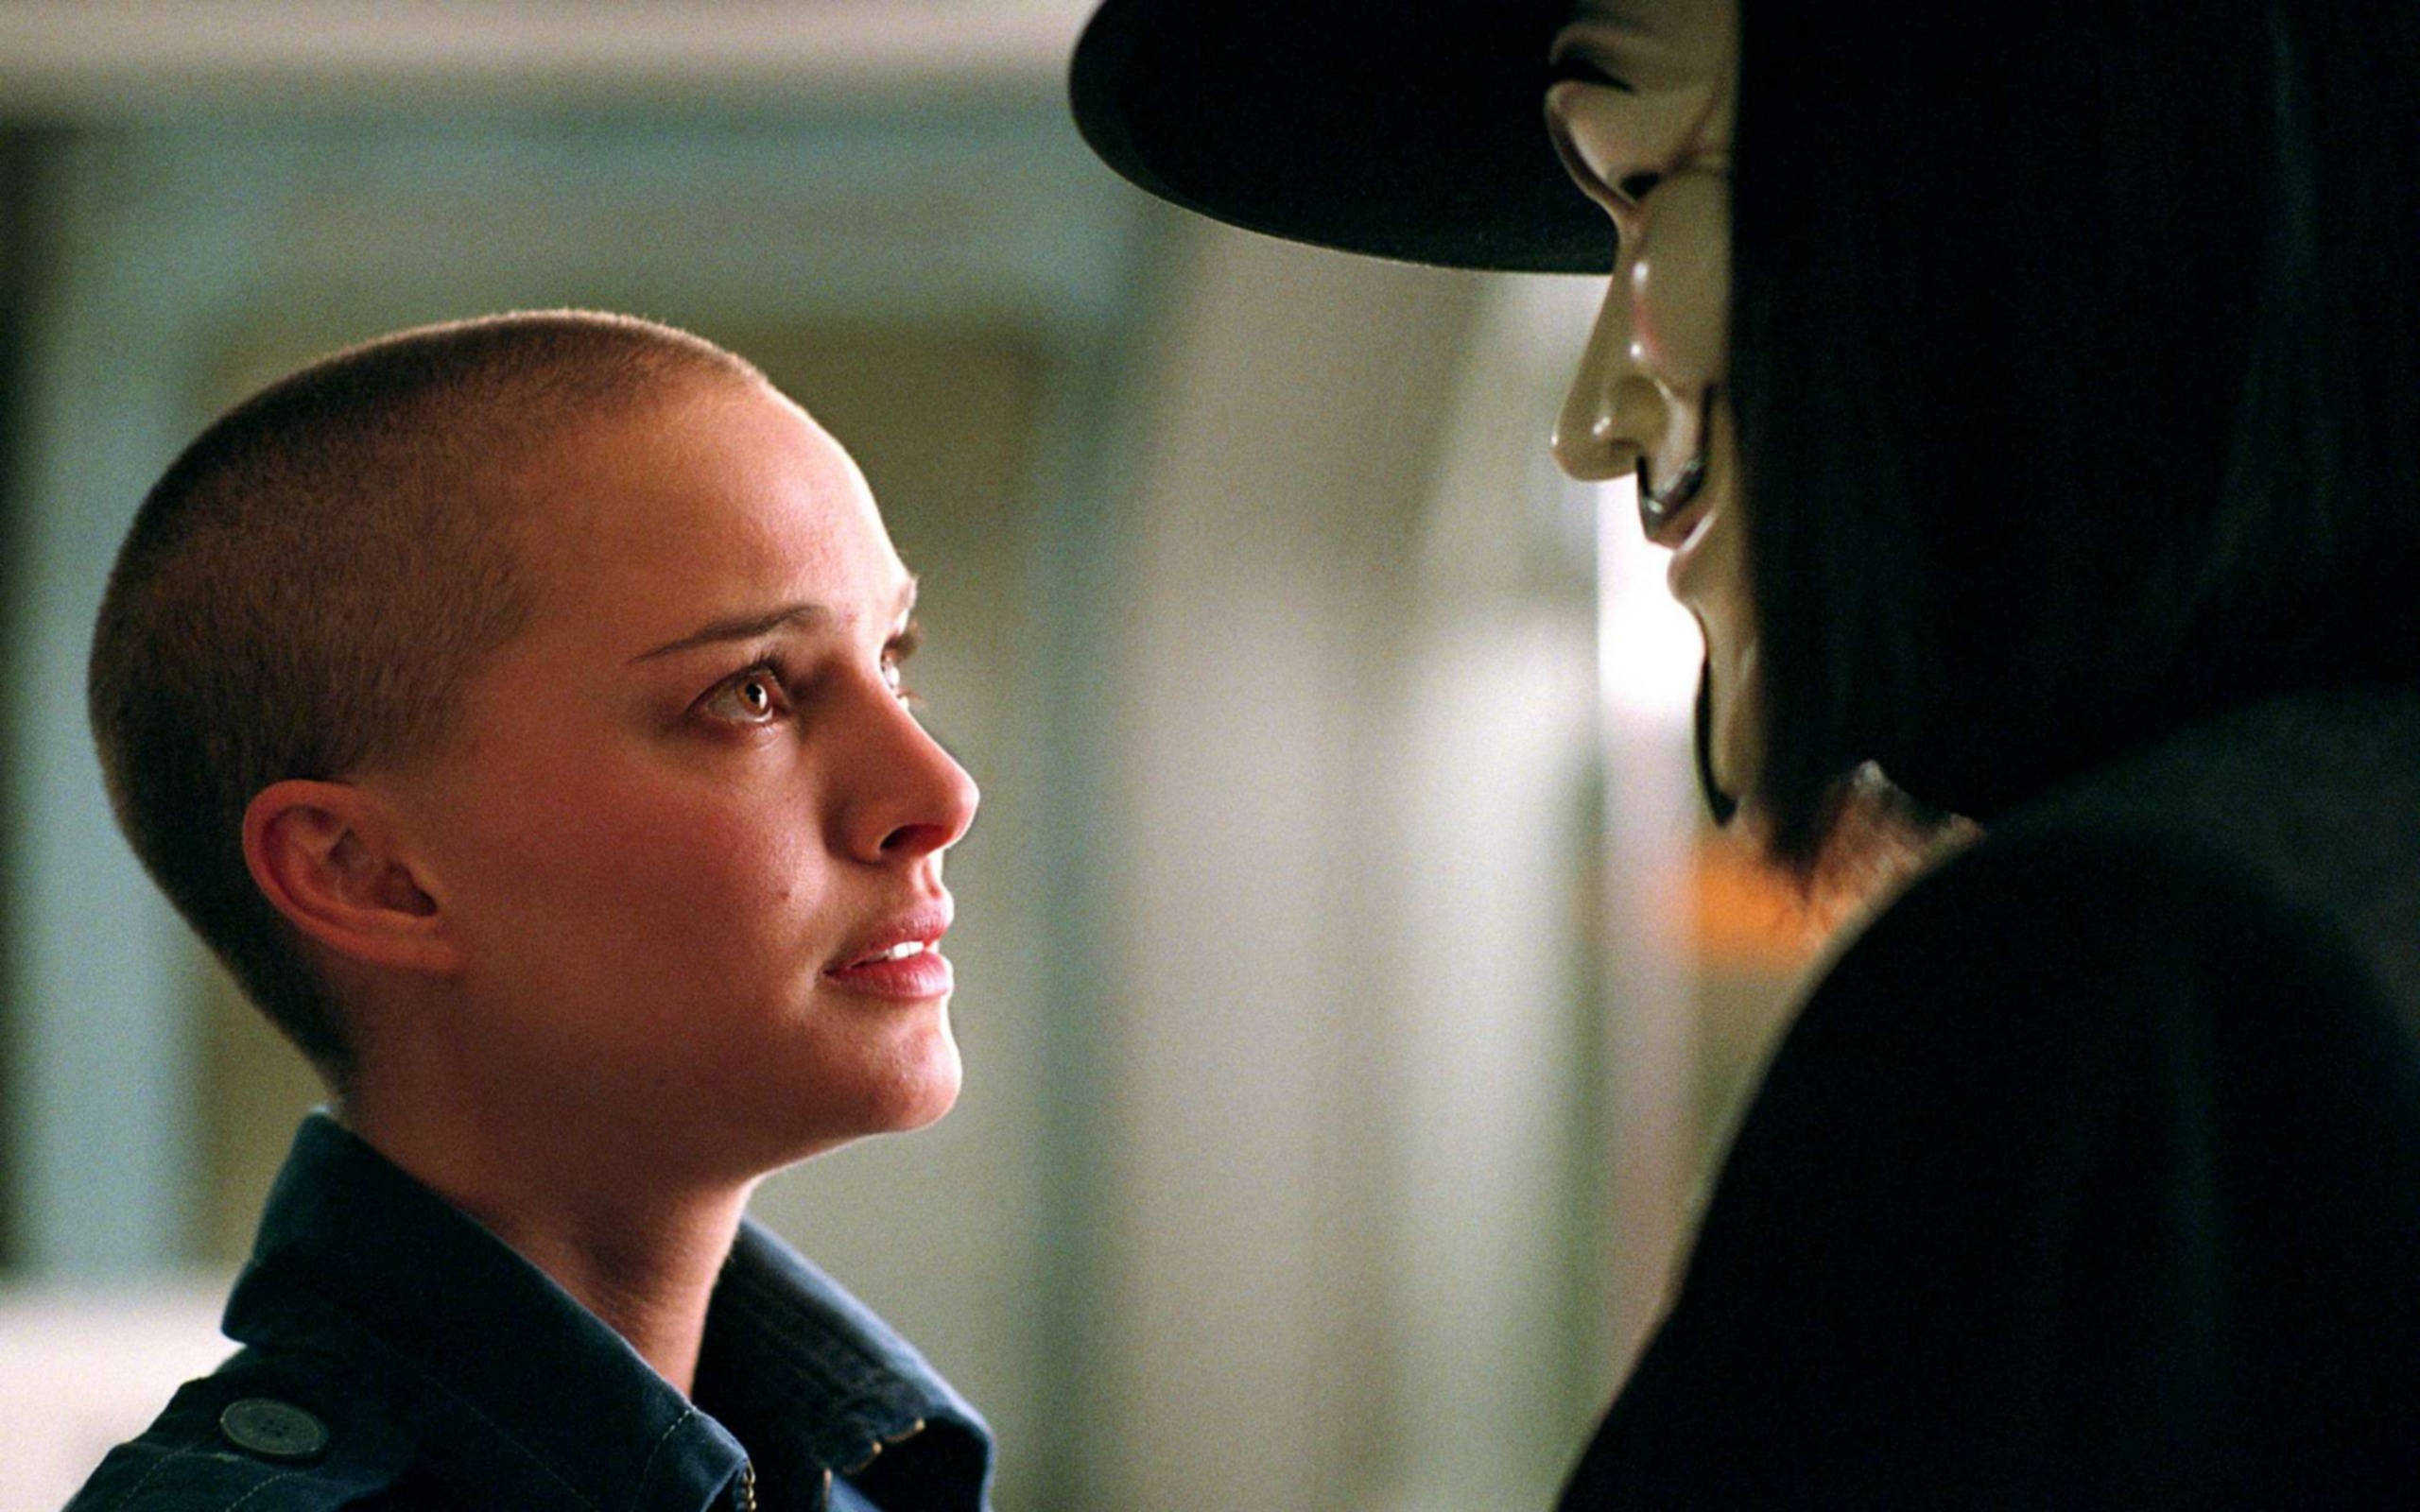
\includegraphics[scale=0.3]{figures/v_for_vendetta-2.jpg}
	\caption{No more trick no more lies only truth..}
\end{figure}
<text> 
\end{frame}

\begin{frame}
	\frametitle{Using Columns with Figures}
	\begin{columns}
		\column{0.5\textwidth}
		<text>
		\column{0.5\textwidth}
\begin{figure}
	
\includegraphics[scale=0.3]{figures/V.jpg}
	\caption{V}
\end{figure}
	\end{columns}
\end{frame}

\section{Julia Code Listings}
\begin{frame}{Julia Source Code Listings}
	\scalebox{1.0}[1.25]{
		\jlinputlisting{./julia_code/add.jl}
	}
\end{frame}





\end{document}